\begin{figure}[p]
\centering
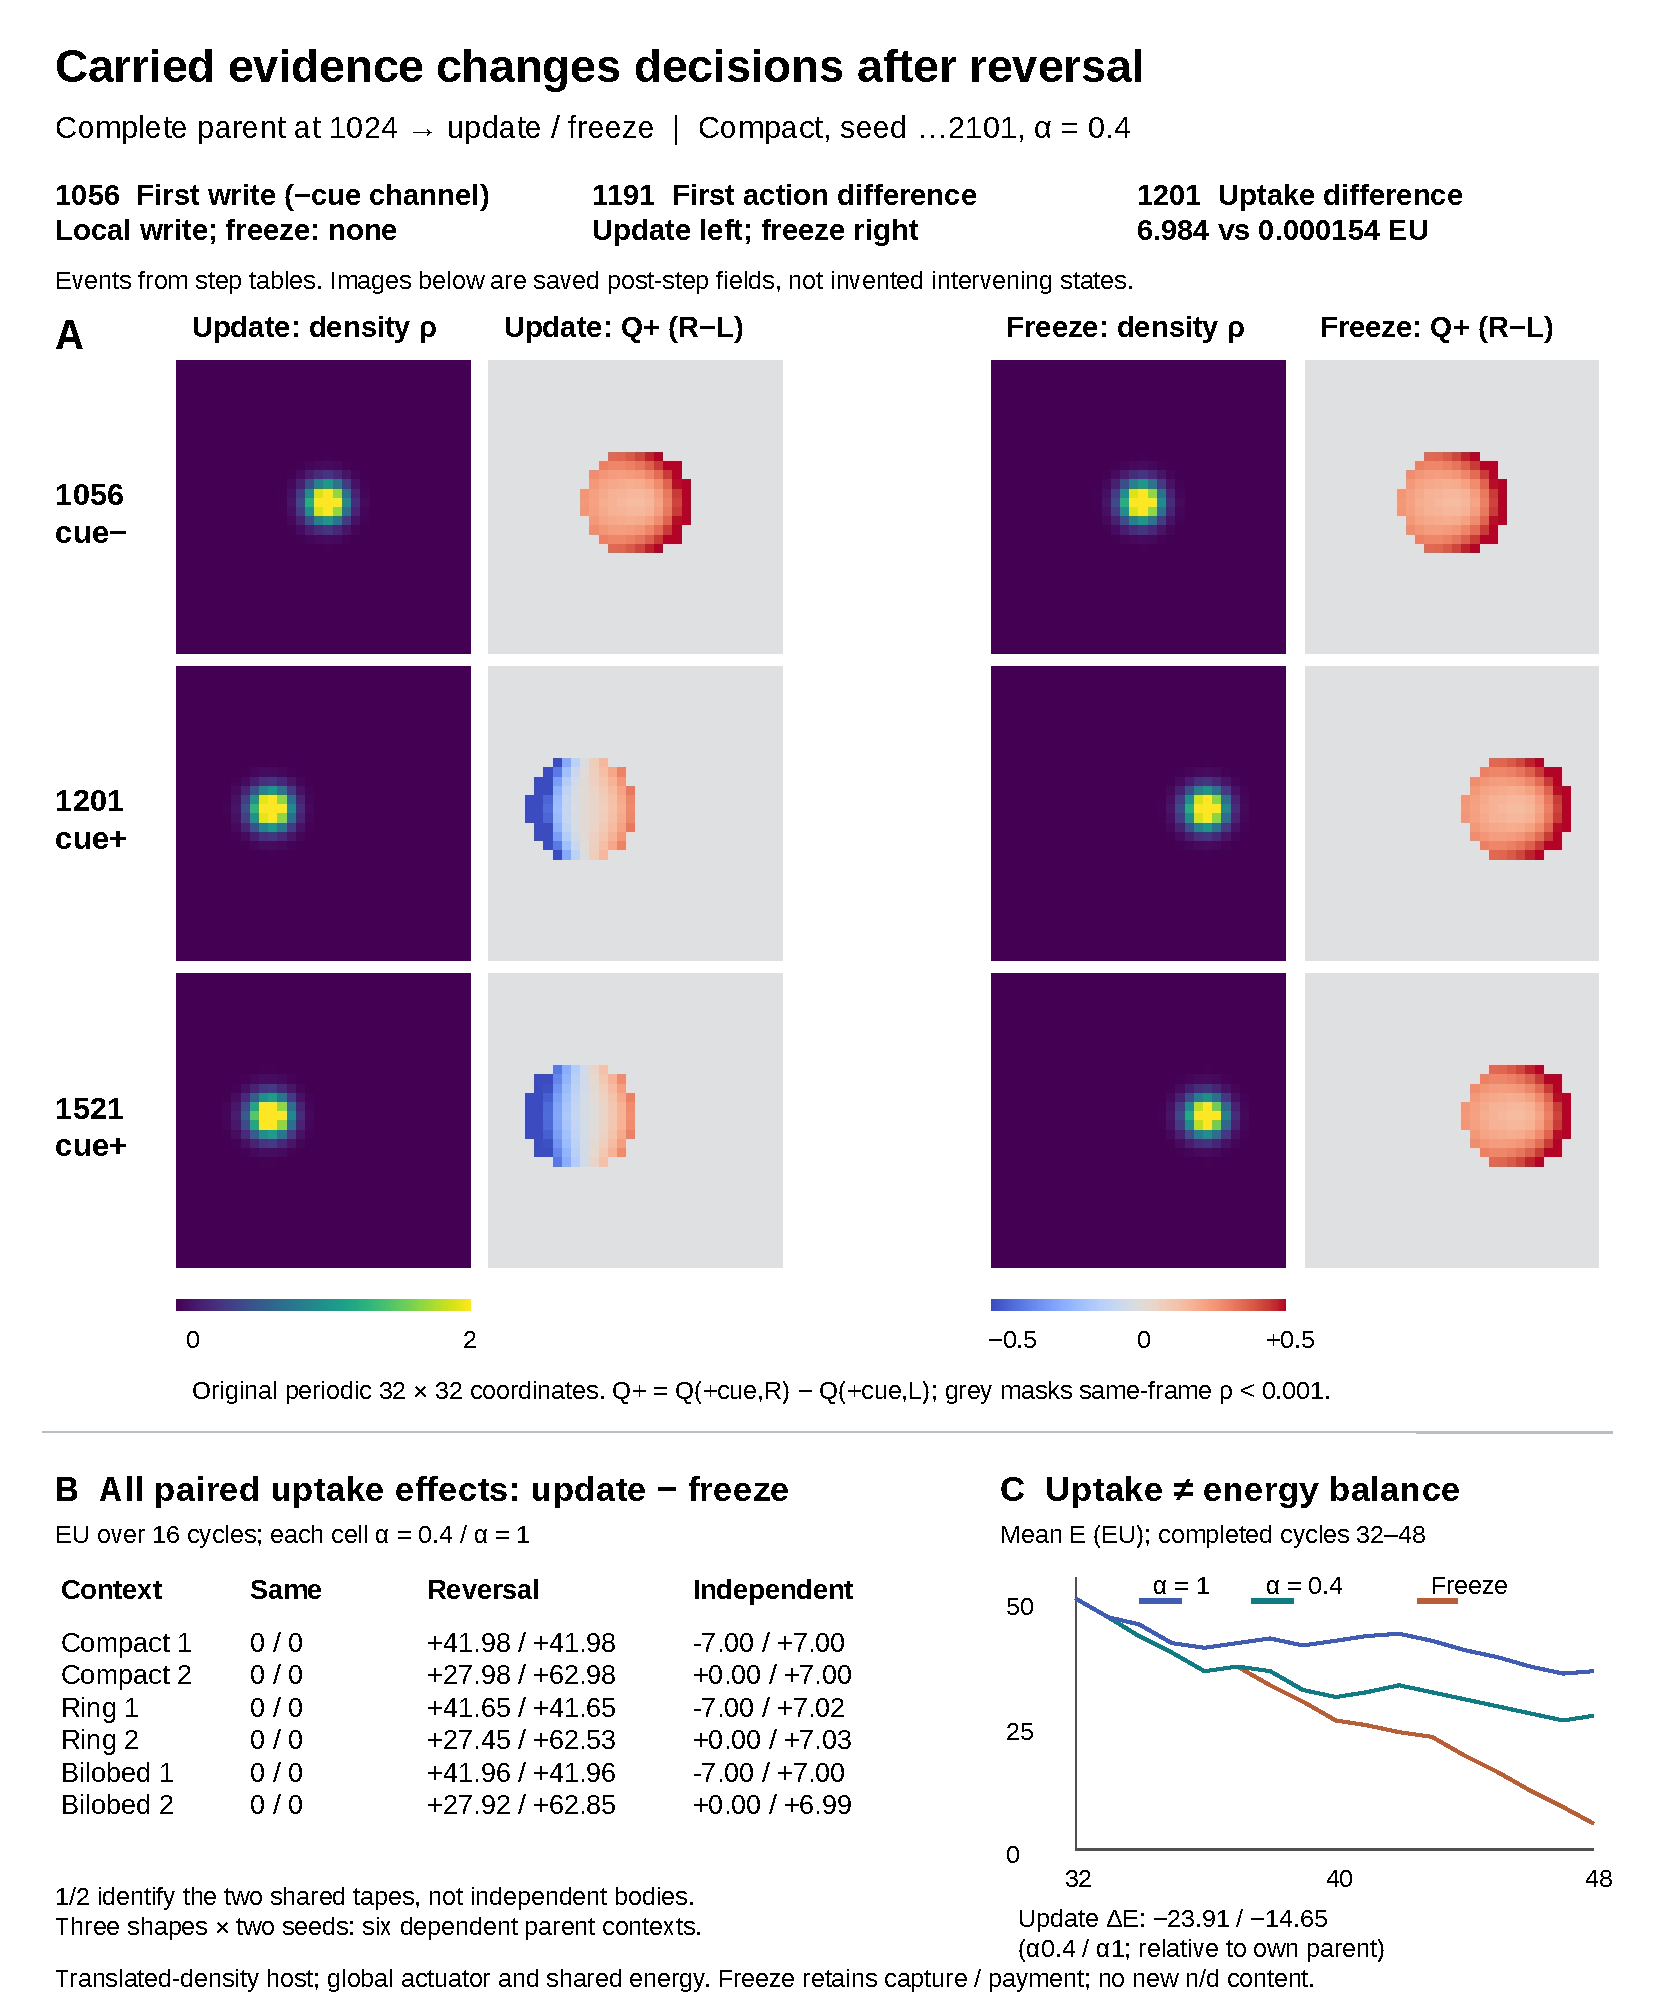
\includegraphics[width=\linewidth,height=0.79\textheight,keepaspectratio]{work/method_renewal/figures/carried_evidence/carried_evidence.pdf}
\captionsetup{font=footnotesize}
\caption{\textbf{Carried evidence changes action after a new reversal without restoring energy balance.}
A compact parent (seed 202610182101, $\alpha=0.4$) branches at step 1024. Logged differences first appear in negative-cue value writing at 1056, action at 1191 and uptake at 1201.
\textbf{a}, Actual saved density and positive-cue value contrast, $q_{+,R}-q_{+,L}$, at steps 1056, 1201 and 1521 for continued updating and paid freezing. Original $32\times32$ coordinates and common scales are retained. Grey masks density below $10^{-3}$; the saved fields lack denominator support, so the mask identifies tissue, not confidence. The first write concerns the negative-cue channel, whereas the stored contrast shows the positive-cue channel. No image at 1191 is inferred.
\textbf{b}, All six shape--seed paired uptake differences under unchanged, reversed and independent mappings, for both update rates. Shapes share two environmental tapes and are not independent histories.
\textbf{c}, Mean reversal-window energy. Updating improves energy relative to freezing, yet both update rates finish below their own parent energy. The faster rate $\alpha=1$ is a strong recent-feedback baseline. These persistent uptake-evidence fields are distinct from the disposable generation-choice channels tested in Table~\ref{tab:material-carried-choice}.}
\label{fig:carried-evidence}
\end{figure}
